\subsection{Decentralized SGF FW Experiments}
To study the performance of Algorithm \ref{decentralized} we used the 10000 images in the MNIST test set, after normalizing them.\\ We split the digit images by giving 10 samples of each class to our 10 workers.
\begin{figure}[htbp]
	\centering
	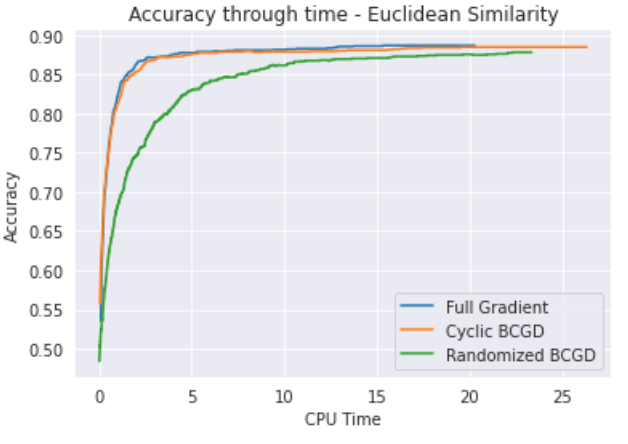
\includegraphics[width=6cm]{accuracy.png}
	\caption{Accuracy of Algorithm \ref{decentralized} with respect to the change on the parameter m.}
	\label{fig:accuracy}
\end{figure}
In Figure \ref{fig:accuracy} we can see a plot in which we represent the behaviour of the Algorithm \ref{decentralized} with respect to the change of the parameter $m$. In particular, we can see that the best value of $m$ who makes the algorithm reaching an accuracy of approximately 20\% is 35, but it is extremely computationally expansive. Fort this reason, we ended up with $m=15$, which is a good compromise between the computation time and the accuracy reached.\\
In our experiments, for each image we estimated its gradient using 20, 50 and 100 queries.\\

\textcolor{gray}{Accuracy error achieved, during the training of the model, the we need to compare the result achieved by testing the model on the whole test set.\\ Notice that the drop of the accuracy, hence the accuracy is discovered already at the 10 epoch/iteration of the algorithms. Comparing the three algorithm is almost the faster one, the competing algorithm in terms of speed convergence of the noise is the distributed.
\\ presence of the pattern in the noise when the accuracy is minimized, more is minimized more the noise the pattern is visible in this algorithms. INstead in the other algorithms the pattern is less visibile e secondo silvia per esempio il variance reduced non presenta un pattern appunto perche il noise e` piu distribuito siccome per la proprieta della varianza considerata nell'algoritmo.
Un piccolo confronto con il guassian noise come fatto nel jupyter sarebbe il top.
}

\begin{figure}
	\centering
	\begin{subfigure}[b]{0.15\textwidth}
		\centering
		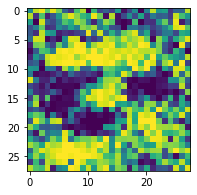
\includegraphics[width=2.5cm]{T20_final.png}
		\caption{}
		\label{fig:decentralized_perturbation_20}
	\end{subfigure}
	\hfill
	\begin{subfigure}[b]{0.15\textwidth}
		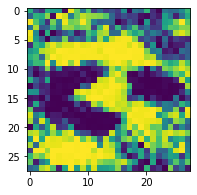
\includegraphics[width=2.5cm]{T50_final.png}
		\caption{}
		\label{fig:decentralized_perturbation_50}
	\end{subfigure}
	\hfill
	\begin{subfigure}[b]{0.15\textwidth}
		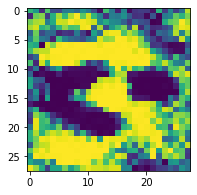
\includegraphics[width=2.5cm]{T100_final.png}
		\caption{}
		\label{fig:decentralized_perturbation_100}
	\end{subfigure}
	\caption{Perturbations of the Decentralized SGF FW algorithm with m=15: \ref{fig:decentralized_perturbation_20} is with T=20, \ref{fig:decentralized_perturbation_50} is with T=50,  \ref{fig:decentralized_perturbation_100} is with T=100.}
	\label{fig:decentralized_perturbations}
\end{figure}
\begin{figure}[h]
	\centering
	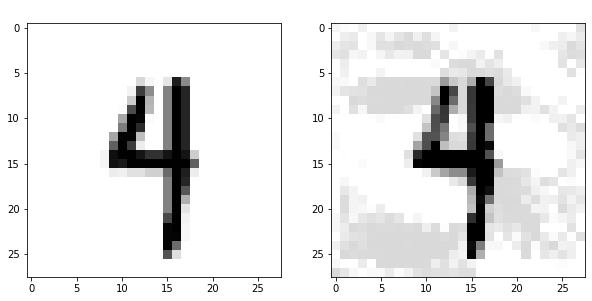
\includegraphics[width=7cm]{image_pertub_T100_final.png}
	\caption{Image of 4 changed to 3 using the best adversarial perturbation generated by the Decentralized Algorithm \ref{decentralized} with a query of 100 and 15 directions.}
	\label{fig:decentralized}
\end{figure}
In Figure \ref{fig:decentralized} we can see an example of the perturbation applyed on an image of the MNIST digits.

\begin{table}[htbp]
	\begin{center}
		\begin{adjustwidth}{-.6cm}{}
			\begin{tabular}{cccc}
				\textbf{Attack} &          20 \textbf{queries} &      50 \textbf{queries} &     100 \textbf{queries} \\
				\midrule
				{\small Decentralized SGF FW}     &    55,25\% &    39,46\% &       36,87\% \\
			\end{tabular}
		\end{adjustwidth}
	\end{center}
	\caption{{\small Summary of $\ell_\infty$ Universal Adversarial Perturbation with $\varepsilon$=0.25. MNIST attack using Decentralized SGF FW. The number of queries is the column denote the nomber of queries used per image.}}
	\label{tab:decentralized}
\end{table}